\documentclass{beamer}
%\usepackage{mdwlist}
\usepackage{graphicx}

\usetheme{Hannover}
\usecolortheme{dolphin}

\usepackage{tikz}
\usetikzlibrary{shadows,positioning,shapes.symbols,fit,arrows,mindmap,trees}

\usepackage{listings}
\lstset{%
    language=Python,               % choose the language of the code
    basicstyle=\ttfamily,          % the size of the fonts that are used for the code
    keywordstyle=\color{blue},
    stringstyle=\color{orange},
    commentstyle=\color{orange},
    numbers=none,                  % where to put the line-numbers
    numberstyle=\footnotesize,     % the size of the fonts that are used for the line-numbers
    stepnumber=2,                  % the step between two line-numbers. If it's 1 each line will be numbered
    numbersep=5pt,                 % how far the line-numbers are from the code
    backgroundcolor=\color{white}, % choose the background color. You must add \usepackage{color}
    showspaces=false,              % show spaces adding particular underscores
    showstringspaces=false,        % underline spaces within strings
    showtabs=false,                % show tabs within strings adding particular underscores
    frame=none,                    % adds a frame around the code
    tabsize=2,                     % sets default tabsize to 2 spaces
    captionpos=b,                  % sets the caption-position to bottom
    breaklines=true,               % sets automatic line breaking
    breakatwhitespace=false,       % sets if automatic breaks should only happen at whitespace
}

% Uncomment this if you use the notes
\usepackage{pgfpages}
\setbeameroption{show notes}                   % Notes on separate page
%\setbeameroption{show notes on second screen} % Page is larger to include notes

% Removes the silly controls
\setbeamertemplate{navigation symbols}{}
% Put slide numbers at the bottom
\setbeamertemplate{footline}[page number]

\title[ServiceSniffer]{Team 11 --- ServiceSNIFFER}
%\subtitle{}
\author[Team 11]{
    Justin Courts \and
    Philip Cristiano \and\\
    Charles Rumford \and
    Thomas Wambold}
\institute[CS493]{Advisor: Dr. William Regli\\CS493\\Drexel University\\\url{http://servicesniffer.net}}
\date{May 25, 2010}

% Do this for notes.
% \note[item]{Baz}

% To include a logo, seems to not work right with all themes
%\logo{\includegraphics[width=3cm]{../logo}}

%%% Tikz stuff %%%
\tikzstyle{box} = [rectangle, drop shadow, rounded corners, minimum height=8mm,
    top color=white, bottom color=blue!30, draw=blue!50!black!100]
\tikzstyle{encbox} = [rectangle, drop shadow, rounded corners,
    top color=white, bottom color=red!30, draw=red!50!black!100]
\tikzstyle{clouds} = [cloud, cloud ignores aspect, cloud puffs=12, draw,
    drop shadow, top color=white, bottom color=blue!30, draw=blue!50!black!100]

\tikzstyle{small mindmap} = [%
    root concept/.style={minimum size=2.3cm,text width=2.1cm,font=\footnotesize},
    level 1 concept/.style={%
        minimum size=1.5cm,
        level distance=2.8cm,
        text width=1.4cm,
        sibling angle=75,
        font=\scriptsize},%
    level 2 concept/.style={%
        minimum size=1.1cm,%
        level distance=2.2cm,%
        text width=1.1cm,%
        sibling angle=60,%
        font=\tiny},%
    level 3 concept/.style={%
        level 2 concept,
        sibling angle=30,%
        font=\tiny},%
    level 4 concept/.style={%
        level 3 concept,
    },
    mindmap,%
    line width=2pt
]

%% End tikz stuff %%%

\begin{document}

%------------------------------------------------------------------------------
%------------------------------------------------------------------------------

\section{Background}
\begin{frame}
    \begin{figure}
        \centering
        \includegraphics[width=.35\textwidth]{../logo}
    \end{figure}
    \vspace{-10mm}
    \titlepage

    \note[item]{Speaker: Charles}
    \note[item]{Your web servers keep crashing and you're not sure why.  You
        have a firewall protecting your network and you run an intrusion
        detection system like Snort, but the servers keep crashing.}

%    \note[item]{ServiceSniffer is a application layer network analyzer which
%    collects traffic off of the network to provide identification of attacks,
%    and analysis and debugging of traffic, concentrated on web services.}
\end{frame}

%------------------------------------------------------------------------------

\subsection{Target Audience}
\begin{frame}{}
    \begin{center}
        \includegraphics[scale=0.5]{503_trimmed.png}
    \end{center}
    \begin{itemize}[<+-| alert@+>]
        \item Your System Administrators:  Uptime!  Uptime!  Uptime!
        \vspace{5mm}
        \item Your Programmers:  No good debugging tools
        \vspace{5mm}
        \item Your Management:  Loss of money/productivity
        \vspace{5mm}
        \item Your Users:  Service interruption
    \end{itemize}

    \note[item]{Speaker: Charles}

    \note[item]{Your systems administrators are worried about their servers going down and blaming the application.}
    \note[item]{Your developers are trying to debug their web services, but there isn't a good tool for this, and they don't believe these crashes are a result of bad code.}
    \note[item]{Your managers are upset about the loss of money and productivity}
    \note[item]{And your users are growing more and more impatient with the interruption of services.  Services they paid you money for, or services they need to do their jobs.}
    \note[item]{But the problem is, you're actually being attacked with a simple Denial of Service attack.  It's just hidden in an XML web service invocation.}
    \note[item]{This is where ServiceSniffer can help you.}
\end{frame}

%------------------------------------------------------------------------------

\subsection{Overview}
\begin{frame}{Overview}
    \begin{itemize}
        \item Application layer
        \vspace{5mm}
        \item Full TCP stream reassembly \& analysis
        \vspace{5mm}
        \item Modular design for extensibility
        \vspace{5mm}
        \item Input and output plug-ins for Snort, SNMP, iptables, etc.
        \vspace{5mm}
        \item Find and act on attacks on web services
    \end{itemize}

    \note[item]{Speaker: Charles}
    \note[item]{ServiceSniffer is an application layer protocol analysis tool
                currently focused on web services.}
    \note[item]{Application layer focuses on process-to-process communication.}
    \note[item]{View the full TCP stream, instead of viewing discrete packets.}
    \note[item]{As you'll see, its modular design allows for easy extensibility.}
    \note[item]{Various input/output plugins allow for interoperability with existing tools.}
\end{frame}

%------------------------------------------------------------------------------

\subsection{Agenda}
\begin{frame}{Agenda}
    \setcounter{tocdepth}{1}
    \tableofcontents
    \setcounter{tocdepth}{3}

    \note[item]{Speaker: Charles}
    \note[item]{An outline of our presentation:  Introduction, Use cases with
                demos, Design, Project Statistic, and Conclusion}
    \note[item]{Introduce: Phil explaining some basics about web service attacks.}
\end{frame}

%------------------------------------------------------------------------------

\subsection{Related Technologies}
\begin{frame}{Related Technologies}
    \begin{itemize}
        \item Web services
        \vspace{5mm}
        \item XML
        \vspace{5mm}
        \item SOAP
        \vspace{5mm}
        \item XML Denial-of-Service (DoS)
    \end{itemize}

    \note[item]{Speaker: Phil}
    \note[item]{Web services: Web APIs accessed via HTTP.}
    \note[item]{XML: Structured markup language.}
    \note[item]{SOAP: XML based web service invocation protocol.}
    \note[item]{XML DoS: We have specifically chosen this attack.  Excessively
        large or difficult to parse structures.  i.e. Deeply nested documents
        can cause problems in parsing.  Mentioned in NSA papers.}
\end{frame}

%------------------------------------------------------------------------------

\subsection{XML DoS Example}
\begin{frame}[fragile]{XML DoS Example - Clean}
    \lstset{language=XML}
    \begin{lstlisting}
<?xml version="1.0"?>
<nutrition>
    <food>
        <name>Truffles</name>
        <calories total="220" fat="170"/>
        <total-fat>19</total-fat>
        <carb>16</carb>
        <protein>1</protein>
    </food>
</nutrition>
    \end{lstlisting}

    \note[item]{Speaker: Phil}
\end{frame}

%------------------------------------------------------------------------------

\begin{frame}[fragile]{XML DoS Example - Nested}
    \lstset{language=XML}
    \begin{lstlisting}
<?xml version="1.0"?>
<nutrition>
    <food>
        <name>Truffles</name>
        <calories total="220" fat="170"/>
        <total-fat>19</total-fat>
        <carb>
            <carb>
                <carb>
                   <!--HERE BE DRAGONS--!>
                </carb>
            </carb>
        </carb>
        <protein>1</protein>
    </food>
</nutrition>
    \end{lstlisting}

    \note[item]{Speaker: Phil}
    \note[item]{Introduce: Justin describing our system design.}
\end{frame}

%------------------------------------------------------------------------------
%------------------------------------------------------------------------------

%\section{Use Cases}
%\begin{frame}{Use Cases}
%    \begin{enumerate}[<+-| alert@+>]
%        \item Reading from a PCAP file to find XML DoS and using iptables to
%            drop the source IP
%        \vspace{5mm}
%        \item Use library interface to find XML DoS to send SNMP traps to
%            a server and dropping the source IP
%        \vspace{5mm}
%        \item Service invocation from the GUI for testing and debugging
%    \end{enumerate}
%
%    \note[item]{Speaker: Tom}
%    \only<1>{
%        \note[item]{
%            For each Use Case Tom is going to demo the system showing how you'd
%            use ServiceSniffer to solve the problem.  He's going to do
%            3 mini-demos -- one for each.}
%        \note[item]{
%            Show opening GUI, loading PCAP file, showing list of services.
%            Show alerts tab.  Show right-click on alert to block IP using
%            iptables.
%    }}
%    \only<2>{\note[item]{
%        This is a demo of the library (CLI) interface.  Show filtering done of
%        the same PCAP.  Show possibility of other inputs.  Show arrangement of
%        processors.
%    }}
%    \only<3>{
%        \note[item]{
%            This is back to the GUI.  Show a regular capture file with SOAP
%            services.  Show the invocations dialog for debugging SOAP services.}
%        \note[item]{Introduce: Justin talking about our system's design
%    }}
%\end{frame}

%------------------------------------------------------------------------------

\subsection{Design Overview}
\begin{frame}{Design Overview}
    \onslide<1->{
       \tikzstyle{kernel} = []
       \tikzstyle{inputs} = []
       \tikzstyle{filproc} = []
       \tikzstyle{outputs} = []
    }
    \only<2>{\tikzstyle{kernel} = [bottom color=orange]}
    \only<3>{\tikzstyle{inputs} = [bottom color=orange]}
    \only<4>{\tikzstyle{filproc} = [bottom color=orange]}
    \only<5>{\tikzstyle{outputs} = [bottom color=orange]}

    \pgfdeclarelayer{background}
    \pgfsetlayers{background,main}

    \begin{tikzpicture}
        \node (invisible) {};
        \node[box, inputs, above=of invisible, xshift=-10]    (pcap) {PCAP File};
        \node[clouds, inputs, below=of invisible, xshift=-10] (net)  {Network};

        \node[box, inputs, right=of invisible]    (capture)    {Capture};
        \node[box, above=of capture]      (storage)    {Storage};
        \node[box, filproc, right=of capture]      (filters)    {Filters};
        \node[box, filproc, right=of filters]      (processors) {Processors};
        \node[box, kernel, below=of filters]      (kernel)     {System Kernel};

        \node[box, outputs, below left=of kernel]  (gui)        {GUI};
        \node[box, outputs, below right=of kernel] (cli)        {CLI};

        \begin{pgfonlayer}{background}
            \node[encbox, draw, fit=(capture)(filters)(processors)(kernel)] (foo) {};
        \end{pgfonlayer}

        \draw[->] (pcap) |- (capture);
        \draw[->] (net) |- (capture);
        \draw[->] (capture) |- (kernel);
        \draw[->] (capture) -- (storage);
        \draw[<->] (filters) -- (kernel);
        \draw[<->] (processors) |- (kernel);
        \draw[<->] (kernel) |- (gui);
        \draw[<->] (kernel) |- (cli);
    \end{tikzpicture}

    \note[item]{Speaker: Justin}
    \note[item]{Describe the modules of the system (Kernel, Inputs, Filters,
                Processors, and Outputs) giving a brief explanation for each of
                them.  Explain how they're coupled together (Queues) and how
                the modularity allows for versatility and extensibility.}
    \note[item]{Each item is arranged in a chain of modules, with data flowing
        from one module to the next via a message-passing queue interface.}
    \note[item]{Kernel: Core of system.  Coordinates data flow from inputs,
        through filters/processors, then to outputs.}
    \note[item]{Inputs: Feed packet data into the system.}
    \note[item]{Filters: Remove data from flow based on some criteria (IP address, etc.)}
    \note[item]{Processors: Transform/add data to the flow.}
    \note[item]{Outputs: Display the data in some form (GUI, CLI, etc.), or
        feed it to another system.}
    \note[item]{Introduce Tom to talk about the demos.}
\end{frame}

%------------------------------------------------------------------------------

\section{Use Cases}
\subsection{Use Case \#1}
\begin{frame}{Use Case \#1}

    Reading from a PCAP file to identify XML DoS attacks.

    \pgfdeclarelayer{background}
    \pgfsetlayers{background,main}
    \begin{center}\begin{tikzpicture}
        \node[box]                   (pcap)       {PCAP File};
        \node[box, below=of pcap]    (capture)    {Capture};
        \node[box, right=of capture] (filters)    {IPFilter};
        \node[box, right=of filters] (processors) {XMLFloodFinder};
        \node[box, below=of filters] (kernel)     {System Kernel};

        \node[box, below=of kernel]  (gui)        {GUI};

        \begin{pgfonlayer}{background}
            \node[encbox, draw, fit=(capture)(filters)(processors)(kernel)] (foo) {};
        \end{pgfonlayer}

        \draw[->] (pcap) -- (capture);
        \draw[->] (capture) |- (kernel);
        \draw[<->] (filters) -- (kernel);
        \draw[<->] (processors) |- (kernel);
        \draw[<->] (kernel) -- (gui);
    \end{tikzpicture}\end{center}

    \note[item]{Speaker: Tom}
     \note[item]{Show opening GUI, loading PCAP file, showing list of services.
         Show alerts tab.}
    \note[item]{Input from a PCAP file}
    \note[item]{Filtering by destination IP for the web server}
    \note[item]{Looking for XML DoS using XMLFloodFinder}
    \note[item]{Output the data to the GUI for analysis}
\end{frame}

%------------------------------------------------------------------------------

\subsection{Use Case \#2}
\begin{frame}{Use Case \#2}

    Snort input plug-in to find XML DoS to send SNMP traps to a server and
    dropping the source IP.

    \pgfdeclarelayer{background}
    \pgfsetlayers{background,main}
    \begin{center}\begin{tikzpicture}
        \node[box]      (capture)       {Snort Plug-in};

        \node[box, above=of capture]        (snort)     {Snort};
        \node[clouds, right=of snort]       (net)       {Network};

        \node[box, right=of capture]        (filters)       {IPFilter};
        \node[box, right=of filters]        (processors)    {XMLFloodFinder};
        \node[box, below=of filters]        (kernel)        {System Kernel};

        \node[box, below left=of kernel]    (snmp)          {SNMPTraps};
        \node[box, below right=of kernel] (iptables)   {iptables};

        \begin{pgfonlayer}{background}
            \node[encbox, draw, fit=(capture)(filters)(processors)(kernel)] (foo) {};
        \end{pgfonlayer}

        \draw[->] (net) -- (snort);
        \draw[->] (snort) -- (capture);
        \draw[->] (capture) |- (kernel);
        \draw[<->] (filters) -- (kernel);
        \draw[<->] (processors) |- (kernel);
        \draw[<->] (kernel) |- (snmp);
        \draw[<->] (kernel) |- (iptables);
    \end{tikzpicture}\end{center}

    \note[item]{Speaker: Tom}
    \note[item]{Input from Snort through a plug-in we developed}
    \note[item]{Filtering by destination IP for the web server - same as before}
    \note[item]{Looking for XML DoS using XMLFloodFinder - same as before}
    \note[item]{Send an SNMPtrap to a server for alerting}
    \note[item]{Add a DROP command to iptables - same as before}
\end{frame}

%------------------------------------------------------------------------------

\subsection{Use Case \#3}
\begin{frame}{Use Case \#3}

    Simple service debugging, viewing list of identified SOAP methods.

    \pgfdeclarelayer{background}
    \pgfsetlayers{background,main}
    \begin{center}\begin{tikzpicture}
        \node[box]      (capture)       {Snort Plug-in};

        \node[box, above=of capture]        (snort)     {Snort};
        \node[clouds, right=of snort]       (net)       {Network};

        \node[box, right=of capture]        (filters)       {HTTP Filter};
        \node[box, right=of filters]        (processors)    {WSDL Filter};
        \node[box, below=of filters]        (kernel)        {System Kernel};

        \node[box, below=of kernel]    (snmp)          {GUI};

        \begin{pgfonlayer}{background}
            \node[encbox, draw, fit=(capture)(filters)(processors)(kernel)] (foo) {};
        \end{pgfonlayer}

        \draw[->] (net) -- (snort);
        \draw[->] (snort) -- (capture);
        \draw[->] (capture) |- (kernel);
        \draw[<->] (filters) -- (kernel);
        \draw[<->] (processors) |- (kernel);
        \draw[<->] (kernel) -- (snmp);
    \end{tikzpicture}\end{center}

    \note[item]{Speaker: Tom}
    \note[item]{Input from Snort through a plug-in we developed}
    \note[item]{Filtering by destination IP for the web server - same as before}
    \note[item]{Looking for XML DoS using XMLFloodFinder - same as before}
    \note[item]{Send an SNMPtrap to a server for alerting}
    \note[item]{Add a DROP command to iptables - same as before}
    \note[item]{Introduce: Phil explaining some aspects of our software
        development process}
\end{frame}

%------------------------------------------------------------------------------

\section{Project Stats}
\subsection{Software Development Tools}
\begin{frame}{Software Development Tools}
    \begin{itemize}
        \item Source Control: Git
        \vspace{5mm}
        \item Build Management: Make and Virtualenv
        \vspace{5mm}
        \item Unit Testing: Nose
        \vspace{5mm}
        \item GUI Wireframing: QtDesigner
    \end{itemize}

    \note[item]{Speaker: Phil}
    \note[item]{Git's distributed model allows us to work offline.  We all know it.}
    \note[item]{Virtualenv is a Python library for managing library versions.
        We used it so we'd have a consistent development environment with
        respect to library versions.}
    \note[item]{Nose is a test-runner for Python's testing framework.  We used
        it for code coverage reports.}
    \note[item]{QtDesigner for wireframing because it allowed for a simple
        drag-and-drop manner of prototyping GUIs, later to be re-done with
        PyQT.}
\end{frame}

%------------------------------------------------------------------------------

\subsection{Testing}
\begin{frame}{Testing}
    \begin{itemize}
        \item Nose: code coverage
        \vspace{5mm}
        \item 88\% code coverage on the library
        \vspace{5mm}
        \item Test cases for each filter/processor.
    \end{itemize}

    \note[item]{Speaker: Phil}
    \note[item]{Message passing allows for easy testing of each
        filter/processor, since we can feed in testing data, and check output.}
\end{frame}

%------------------------------------------------------------------------------
%------------------------------------------------------------------------------

\section{Conclusion}
\subsection{Alternative Products}
\begin{frame}{Alternative Products}
    \begin{itemize}
        \item \textbf{Wireshark} - Cumbersome, manual process
        \vspace{5mm}
        \item \textbf{Snort} - Lower layer NIDS
        \vspace{5mm}
        \item \textbf{Nagios} - Notification framework
    \end{itemize}

    \note[item]{Speaker: Phil}
    \note[item]{\textbf{Wireshark}:  Data is available to determine this data,
                but it would need to be gotten manually.  Wireshark not
                designed for automated tasks and analysis of fully reassembled
                TCP streams}
    \note[item]{\textbf{Snort}:  Way too clunky and bloated to use, and
                requires a domain-specific language to be learned just to use
                it}
    \note[item]{\textbf{Nagios}:  Lower layer notification framework designed
                more for event triggers than analysis}
    \note[item]{Introduce: Justin to wrap-up}
\end{frame}

%------------------------------------------------------------------------------

\subsection{Components}
\begin{frame}{Components}
    \pgfdeclarelayer{background}
    \pgfsetlayers{background,main}
    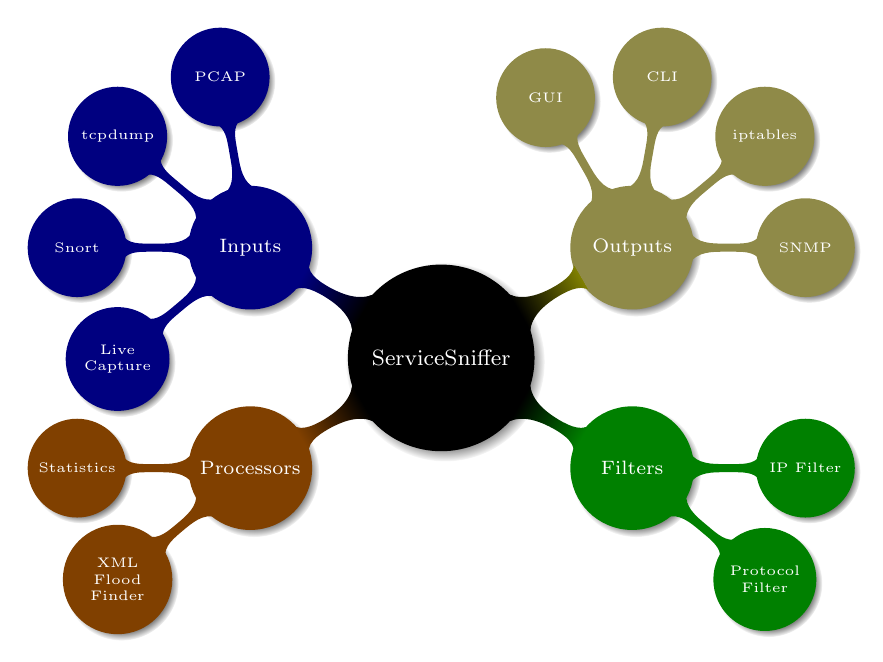
\begin{tikzpicture}[small mindmap,
            every node/.style={concept, circular drop shadow},
            text=white,
        ]
        \node {ServiceSniffer}
            child[grow=150, concept color=blue!50!black] { node {Inputs}
                child[grow=100] { node {PCAP}         }
                child[grow=140] { node {tcpdump}      }
                child[grow=180] { node {Snort}        }
                child[grow=220] { node {Live Capture} }
            }
            child[grow=210, concept color=orange!50!black] { node {Processors}
                child[grow=180] { node {Statistics}       }
                child[grow=220] { node {XML Flood Finder} }
            }
            child[grow=330, concept color=green!50!black] { node {Filters}
                child[grow=0]   { node {IP Filter}       }
                child[grow=320] { node {Protocol Filter} }
            }
            child[grow=30, concept color=yellow!50!black] { node {Outputs}
                child[grow=120] { node {GUI}      }
                child[grow=80]  { node {CLI}      }
                child[grow=40]  { node {iptables} }
                child[grow=0]   { node {SNMP}     }
            }
        ;
    \end{tikzpicture}
    \note[item]{Speaker: Justin}
    \note[item]{Re-state how everything fits together producing a modular
        program which can easily interoperate with other tools you use.}
\end{frame}

%------------------------------------------------------------------------------

\subsection{Wrap-up}
\begin{frame}{Wrap-up}
    \begin{itemize}
        \item New protocols --- XMPP or non-web service protocols
        \vspace{5mm}
        \item New interfaces --- Mobile Client, Application Plug-ins
        \vspace{5mm}
        \item New filters/processors --- Protocol specific processing
    \end{itemize}

    \note[item]{Speaker: Justin}
    \note[item]{Quick refresh of the major points:  Modularity, Extensibility,
                etc.  Each of these allow us to add new things easily.}
\end{frame}

%------------------------------------------------------------------------------

\subsection{Questions?}
\begin{frame}{Questions?}
    \begin{itemize}
        \item See our website at \url{http://servicesniffer.net}
        \vspace{10mm}
        \item Can send questions to \url{list@servicesniffer.net}
    \end{itemize}
    \note[item]{Speaker: Justin}
\end{frame}

%------------------------------------------------------------------------------

\end{document}
